\documentclass{article}

\usepackage[margin=1in]{geometry}     %for 1inch margins that play nice with fancyhdr
\usepackage{amsmath,amssymb}          % math and junk
\usepackage{fancyhdr}                 % for a nice running header and footer
\usepackage{lastpage}                 % for nice "X of Y" footer
\usepackage[per-mode=symbol,alsoload=binary,detect-all=true]{siunitx}
                                      % for nice units and junk!
\usepackage{gnuplot-lua-tikz}         % enable tikz plots made from gnuplot
\usepackage{float}                    % [H] option for floats
\usepackage[american]{circuitikz}     % for teh circuit diagrams
\usepackage[hidelinks]{hyperref}                 % get those sweet, sweet, links
\usepackage{framed}                   % for framed titlepage
\usepackage{subfig}

\usetikzlibrary{shapes,arrows}

% unused, but common for other experiments
%\usepackage{rotating}                 % for sideways stuff!
%\usepackage{cancel}                   % for `canceling out' parts of equations. fancy!
\usepackage{mdwlist}                  % itemize* and friends
%\usepackage{verbatim}                 % for \verbatiminput command and comment environment
%\usepackage[colorinlistoftodos]{todonotes}                % todo's, if used/needed
%\usepackage{multirow}                 % for multi-row spans in tabular environment


% values!
\newcommand{\docAuthor}{Sean Barag}
\newcommand{\docCoAuthor}{None}
\newcommand{\ta}{Yang Gao}
\newcommand{\docTitle}{Building the ADC Circuit}
\newcommand{\courseName}{ECE-L304}
\newcommand{\labNum}{Step 2}
\newcommand{\labSec}{064}
\newcommand{\dueDate}{3 January 2012}
\newcommand{\perfDate}{18 \& 25 January 2012}

% paths
\graphicspath{{$HOME/texmf/graphics/}}


% meta-data
\pdfinfo{
	/Title    (\labNum: \docTitle)
	/Author   (\docAuthor)
	/Keywords (\docTitle, \labNum)
}

% for fancy header
\pagestyle{fancy}
\lhead{\courseName\ $|$ \labSec}
\chead{\labNum: \docTitle}
\rhead{\docAuthor}
\cfoot{\thepage\ of \pageref{LastPage}}

% title info
\title{\courseName\ \labNum: \\ \docTitle}
\author{\docAuthor}
\date{}

% shortcuts, cause I'm lazy
\newcommand{\bs}[1]{\boldsymbol{#1}}
\newcommand{\tbf}[1]{\textbf{#1}}
\newcommand{\ttt}[1]{\texttt{#1}}

\begin{document}
% Cover page written by Bryndon Blackburn
% Originally written by Bryndon Blalckburn
\begin{titlepage}
	\begin{center}
		\includegraphics[scale = 0.50]{DrexelLogo.pdf}
	\end{center}

	\large
	\begin{framed}
		\begin{center}
			Electrical and Computer Engineering Dept. \\
			Electrical Engineering Laboratory IV, ECE-L304 \\
		\end{center}
	\end{framed} \vspace{50pt}

	\begin{description}
		\item[Title:]\labNum: \docTitle
		\item[Author:] \docAuthor
		\item[Partner:] \docCoAuthor
		\item[Instructor:] \ta
		\item[Section:] \labSec
		\item[Date Performed:] \perfDate
		\item[Date Due:] \dueDate
		\item[Date Received:]
	\end{description}
\end{titlepage}


% Blank page so two-sided printing leaves the cover page on its own sheet
\thispagestyle{empty}
\newpage
\mbox{}

\maketitle
\setcounter{page}{1} % fixes page numbering issues caused by cover sheet
\tableofcontents % this helps
\newpage
\listoffigures   % there's over 9000 figures

\newpage % I want the actual content to be at the top of a new page

\section{Introduction}
The entirety of ECE-L304 is devoted to the design, construction, and debugging
of a digital voice recorder.  By providing students with an opportunity to
complete a project of larger scale than anything they have previously
attempted, the course offers its students valuable skills and experience with a
long-term engineering project.

As the system uses digital storage in the form of a RAM chip, it is necessary
to convert all input audio from its native analog form to a digital
representation.  Similarly, the stored digital representation must be converted
back to an analog signal so that it can be correctly rendered by a speaker.
These conversions are performed by an analog to digital converter (ADC) and a
digital to analog converter (DAC), resepectively.
%
In order to ease the design process, students first complete a simple ADC and
DAC simulation.  This helps to remind students of the operating properties and
behaviors of the two converters, as well as providing a schematic similar to
the one required in the final design.

\section{Elements}

After consulting the datasheet for the DAC0808 integrated circuit, it was
determined that three~\SI{5}{\kilo\ohm} resistors were required for the proper
operation of the chip.  The measured values are shown in
Table~\ref{t:elements}, along with the elements used in the construction of the
ADC in step 2 (which utilized the ADC0804 IC).
%
\begin{table}[H]
\centering
	\section{Elements}

After consulting the datasheet for the DAC0808 integrated circuit, it was
determined that three~\SI{5}{\kilo\ohm} resistors were required for the proper
operation of the chip.  The measured values are shown in
Table~\ref{t:elements}, along with the elements used in the construction of the
ADC in step 2 (which utilized the ADC0804 IC).
%
\begin{table}[H]
\centering
	\section{Elements}

After consulting the datasheet for the DAC0808 integrated circuit, it was
determined that three~\SI{5}{\kilo\ohm} resistors were required for the proper
operation of the chip.  The measured values are shown in
Table~\ref{t:elements}, along with the elements used in the construction of the
ADC in step 2 (which utilized the ADC0804 IC).
%
\begin{table}[H]
\centering
	\input{tbl/elements.tex}
	\parbox{.8\textwidth}{
	\caption[List of used elements]{Required, nominal, and measured element
	values used in the ADC and DAC circuits.}
	\label{t:elements}}
\end{table}
%
With errors for the DAC resistors all falling under~\SI{1}{\percent}, the
elements are all appropriately accurate for this application.

	\parbox{.8\textwidth}{
	\caption[List of used elements]{Required, nominal, and measured element
	values used in the ADC and DAC circuits.}
	\label{t:elements}}
\end{table}
%
With errors for the DAC resistors all falling under~\SI{1}{\percent}, the
elements are all appropriately accurate for this application.

	\parbox{.8\textwidth}{
	\caption[List of used elements]{Required, nominal, and measured element
	values used in the ADC and DAC circuits.}
	\label{t:elements}}
\end{table}
%
With errors for the DAC resistors all falling under~\SI{1}{\percent}, the
elements are all appropriately accurate for this application.

\section{Clock Frequency Measurement}
After installing the resistor and capacitor in the appropriate terminals, the
system was powered with zero input so that students could observe the waveform
that appeared at pin four of the ADC, i.e. the internal clock frequency.  An
oscilloscope screenshot of this signal is shown in Figure~\ref{f:clock}.
%
\begin{figure}[H]
\centering
	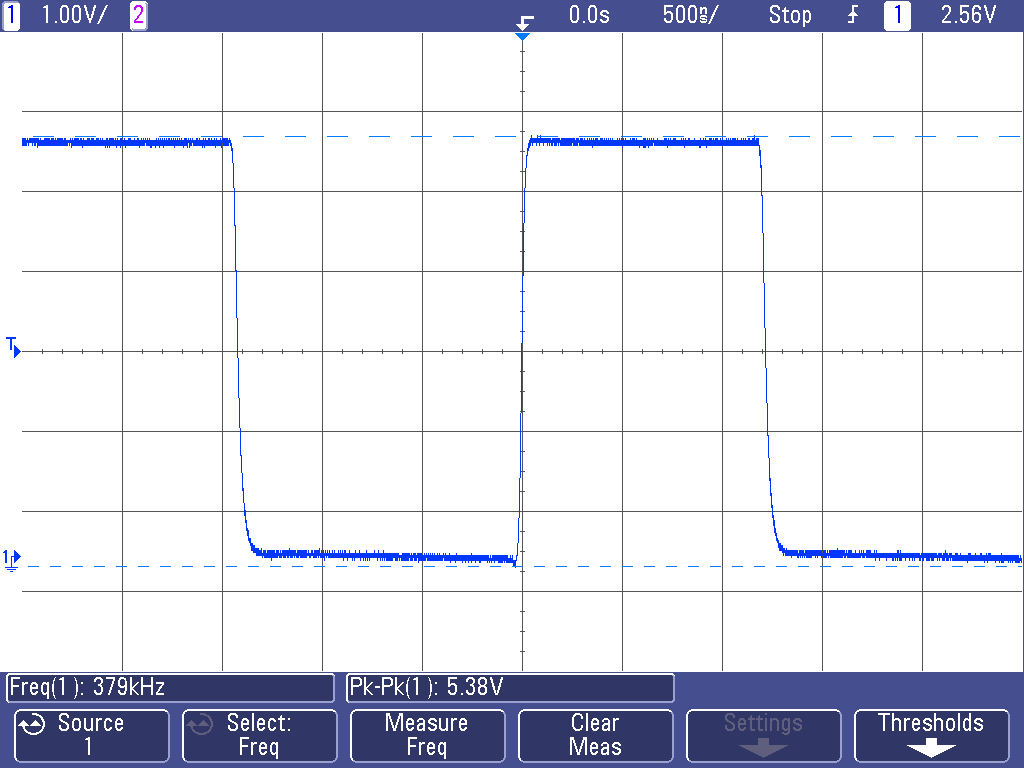
\includegraphics[width=.8\textwidth]{img/shot/RC_clock_shot.png}
	\parbox{.8\textwidth}{
	\caption[Internal clock waveform]{Captured signal of the system's internal
	clock.  Note the drastic decrease in frequency compared to the target
	frequency.}
	\label{f:clock}}
\end{figure}
%
As is shown, the clock frequency of the ADC is only about half of the intended
frequency.  This is most easily attributed to additional intrinsic capacitances
within the circuit board.  Despite the severely decreased clock frequency, all
other students observed a similar phenomenon in their systems, and the
instructor confirmed that this is a known flaw in the design.  As such, the
evaluation of the ADC was allowed to proceed with an internal clock frequency
of~\SI{379}{\kilo\hertz}.

\section{Conclusions}

In conclusion, students simulated a fully functional RAM system in which data
was both stored to and retrieved from the~\SI{64}{kb} RAM chip.   Both the
rudimentary and complex systems exhibited the correct timing behavior, and
reproduced the input data accurately.  While the output of the 8-bit system in
part two showed some anomalies, they are acceptable for the purposes of a basic
voice recorder.  After tuning the complex design so that the anomalies were of
a safe voltage, both systems are ready to be implemented in hardware.


\newpage
\appendix
\section{License}
\section{License}

Copyright \copyright\ 2011, Sean Barag.  All rights reserved.

Redistribution and use in source and binary forms, with or without
modification, are permitted provided that the following conditions are met:
\begin{itemize}
\item Redistributions of source code must retain the above copyright notice, this
  list of conditions and the following disclaimer.
\item Redistributions in binary form must reproduce the above copyright notice, this
  list of conditions and the following disclaimer in the documentation and/or
  other materials provided with the distribution.
\item Neither the name of the owner nor the names of its contributors may be
  used to endorse or promote products derived from this software without specific
  prior written permission.
\end{itemize}

THIS SOFTWARE IS PROVIDED BY THE COPYRIGHT HOLDERS AND CONTRIBUTORS ``AS IS'' AND
ANY EXPRESS OR IMPLIED WARRANTIES, INCLUDING, BUT NOT LIMITED TO, THE IMPLIED
WARRANTIES OF MERCHANTABILITY AND FITNESS FOR A PARTICULAR PURPOSE ARE
DISCLAIMED. IN NO EVENT SHALL THE COPYRIGHT HOLDER OR CONTRIBUTORS BE LIABLE
FOR ANY DIRECT, INDIRECT, INCIDENTAL, SPECIAL, EXEMPLARY, OR CONSEQUENTIAL
DAMAGES (INCLUDING, BUT NOT LIMITED TO, PROCUREMENT OF SUBSTITUTE GOODS OR
SERVICES; LOSS OF USE, DATA, OR PROFITS; OR BUSINESS INTERRUPTION) HOWEVER
CAUSED AND ON ANY THEORY OF LIABILITY, WHETHER IN CONTRACT, STRICT LIABILITY,
OR TORT (INCLUDING NEGLIGENCE OR OTHERWISE) ARISING IN ANY WAY OUT OF THE USE
OF THIS SOFTWARE, EVEN IF ADVISED OF THE POSSIBILITY OF SUCH DAMAGE.\\

Source code for this document is available at \texttt{http://github.com/sjbarag/}.


\end{document}
